\documentclass[14pt,fleqn]{extarticle}
\usepackage[T2A,T1]{fontenc}
\usepackage[utf8]{inputenc}
\usepackage[russian]{babel}
\usepackage{amsmath}
\usepackage{graphicx}
\usepackage{tabularx}
\usepackage{boldline}
\usepackage{makecell}
\usepackage{arydshln}
\usepackage{mathtools}
\usepackage{centernot}
\usepackage[a4paper, total={6.5in, 9.5in}]{geometry}

\graphicspath{ {./images/} }
\setlength{\mathindent}{0pt}
\setlength\parindent{0pt}

\def\at{
	\left.
	\vphantom{\int}
	\right|
}


\begin{document}
	\begin{titlepage}
		
\includegraphics[scale=0.12]{logo}
		\begin{center}
			\textbf{МИНОБРНАУКИ РОССИИ}\\
			\vspace{0.2cm}
			\textbf{Федеральное государственное бюджетное образовательное учреждение высшего образования}\\
			\textbf{<<САНКТ-ПЕТЕРБУРГСКИЙ ГОСУДАРСТВЕННЫЙ ЭКОНОМИЧЕСКИЙ УНИВЕРСИТЕТ>>}\\
			\vspace{0.6cm}
			Факультет информатики и прикладной математики\\
			Кафедра прикладной математики и экономико-математических методов\\
			\vspace{1cm}
			\textbf{ОТЧЁТ}\\
			по дисциплине:\\
			\textbf{<<Имитационное моделирование>>}\\
			на тему:\\
			\textbf{<<Треугольное распределение. Задание №1>>}\\
		\end{center}
		\vspace{1cm}
		Направление: 01.03.02\\
		Обучающийся: Бронников Егор Игоревич\\
		Группа: ПМ-1901\\
		\vfill
		\begin{center}
			Санкт-Петербург\\
			2022\\
		\end{center}
	\end{titlepage}
    \subsection*{Задание}
    Получить аналитическое выражение для функции распределения $F(x)$ треугольного закона с параметрами $a$ (\textit{min}), $b$ (\textit{max}), $c$ (\textit{мода}). Найти аналитическое выражение для обратной функции $F^{-1}(x)$.
    \begin{figure}[h]
        \centering 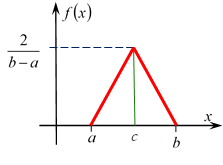
\includegraphics[scale=0.8]{plot}
        \caption{График плотности треугольного закона}
    \end{figure}
    \subsection*{Решение}
    \subsubsection*{Плотность распределения $f(x)$}
    Уравнение по двум точкам:
    \begin{center}
        $\dfrac{y-y_1}{y_2-y_1} = \dfrac{x-x_1}{x_2-x_1} \quad \Rightarrow \quad y = \dfrac{x-x_1}{x_2-x_1} \cdot (y_2-y_1) + y_1$
    \end{center}
    
    1) Рассмотрим случай $x \in [a, c]$:\\
    \newline
    Точки: $\left(a, 0\right), \left(c, \dfrac{2}{b-a}\right)$
    \begin{center}
        $f_1(x) = \dfrac{x-a}{c-a} \cdot \left(\dfrac{2}{b-a} - 0\right) + 0 \quad \Rightarrow \quad f_1(x) = \dfrac{2(x-a)}{(b-a)(c-a)}$
    \end{center}
    
    2) Рассмотрим случай $x \in [c, b]$:\\
    \newline
    Точки: $\left(c, \dfrac{2}{b-a}\right), \left(b, 0\right)$
    \begin{center}
        $f_2(x) = \dfrac{x-c}{b-c} \cdot \left(0 - \dfrac{2}{b-a}\right) + \dfrac{2}{b-a} \quad \Rightarrow \quad f_2(x) = \dfrac{2(b-x)}{(b-c)(b-a)}$
    \end{center}

    \newpage
    
    \textit{Плотность треугольного распределения}:
    \begin{align*}
        f(x) =
        \begin{cases}
            \dfrac{2(x-a)}{(b-a)(c-a)} \quad , x \in [a,c]\\
            \dfrac{2(b-x)}{(b-c)(b-a)} \quad , x \in [c,b]\\
            0 \hspace{3.25cm} , x \centernot\in [a,b]\\
        \end{cases}
    \end{align*}
    
    \subsubsection*{Функция распределения $F(x)$}

    По свойству функции распределения: $f'(x) = F(x)$.\\

    1) Рассмотрим случай $x \in [a,c]:$
    \[ F_1(x) = \int_{a}^{x} \dfrac{2(t-a)}{(b-a)(c-a)} \,dt = \dfrac{t(t-2a)}{(b-a)(c-a)}\at_{a}^{x} = \dfrac{(x-a)^2}{(b-a)(c-a)} \]
    
    2) Рассмотрим случай $x \in [c,b]$:\\
    \newline
    При вычислении функции распределения на этом участке следует помнить, что у нас был предшествующий отрезок от $[a,c]$, тогда нужно посчитать его площадь и прибавить к $F_2(x)$.
    \[ F_1(c) = \dfrac{c-a}{b-a}\]
    \[ F_2(x) = \dfrac{c-a}{b-a} + \int_{c}^{x} \dfrac{2(b-t)}{(b-c)(b-a)} \,dt = \dfrac{c-a}{b-a} + \dfrac{t(2b-t)}{(b-c)(b-a)}\at_{c}^{x} = \]
    \[ = \dfrac{c-a}{b-a} + \dfrac{(2b-c-x)(x-c)}{(b-a)(b-c)} = 1 - \dfrac{(x-b)^2}{(b-a)(b-c)} \]
    \newline
    \textit{Функция распределения треугольного закона}:
    \begin{align*}
        F(x) =
        \begin{cases}
            0 \hspace{4.1cm} , x < a\\
            \dfrac{(x-a)^2}{(b-a)(c-a)} \hspace{1.3cm} , x \in [a,c]\\
            1 - \dfrac{(x-b)^2}{(b-a)(b-c)} \quad , x \in [c,b]\\
            1 \hspace{4.1cm} , x > b\\
        \end{cases}
    \end{align*}
   
    \newpage
    \begin{figure}[h]
        \centering 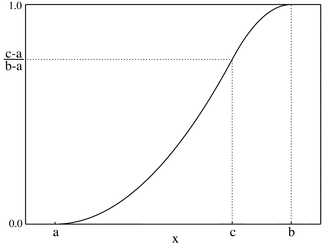
\includegraphics[scale=0.8]{plot2}
        \caption{График функции распределения треугольного закона}
    \end{figure}

    \subsubsection*{Обратная функция $F^{-1}(x)$}
    
    У функции распределения есть ограничение: $0 < F(x) < 1$, которое стоит учитывать.\\
    Пусть $y = F(x)$\\
    \newline
    1) Рассмотрим случай $0 < y < \dfrac{c-a}{b-a}$:
    \[ F_1^{-1}(y) = x_1 = a + \sqrt{(b-a)(c-a)y} \]
    
    2) Рассмотрим случай $\dfrac{c-a}{b-a} \leq y < 1$:
    \[ F_2^{-1}(y) = x_2 = b - \sqrt{(b-a)(b-c)(1-y)} \]

    \textit{Обратная функция} $F^{-1}(x)$:
    \begin{align*}
        F^{-1}(y) = x =
        \begin{cases}
            a + \sqrt{(b-a)(c-a)y} \hspace{2.2cm} , 0 < y < \dfrac{c-a}{b-a}\\
            b - \sqrt{(b-a)(b-c)(1-y)} \hspace{1cm} , \dfrac{c-a}{b-a} < y < 1\\
        \end{cases}
    \end{align*}
\end{document}
